% Need to fix optimization problems -- add spacing between min and obj
% Derive analytic min cut bipartition formula using Lagrangian multipli
%#######################################################################

In this chapter we introduce a different approach to the graph
partitioning problem. Rather than use local search heuristics to find
candidate partitions and evaluate them using pre-defined criteria, the
optimization approach uses or adapts one or more of the validation
criteria in chapter 2 as an objective function and seeks to maximize or
minimize this objective using the vertex partition assignments as
decision variables.

We will start with a simple idea to frame the brain parcellation task as
an optimization problem. We will then repeatedly refine the optimization
problem to let it satisfy our notions of what constitutes a good
parcellation and be computationally tractable. 

For all edges $(i,j) \in E$, let $w_{ij}$ denote the weight of the edge
connecting vertices $i$ and $j$.

\begin{definition}
Adjacency matrix. $A \in \mathcal{S}^n$
\[
A_{ij} = \begin{cases}
  w_{ij} & \text{if} (i,j) \in E \\
  0      & \text{otherwise} \\
\end{cases}
\]
\end{definition}

\begin{definition}
Degree matrix. $D \in \mathcal{S}^n$
\[
D_{ij} = \begin{cases}
  \sum_{k = 1}^n A_{ik} & \text{if} i = j \\
  0                     & \text{otherwise} \\
\end{cases}
\]
\end{definition}

\section{Edge Weight Minimizing Bipartition}

In the previous chapter, we showed how local search heuristics produced
parcels that were balanced and had high within-parcel and low between-
parcel edge weights. However, one salient issue with these parcellations
was lack of smoothness, or regularity in the parcels' spatial shapes.

An effective way of encouraging parcel smoothness is to minimize the sum
of weights on all edges connecting a parcel to a different parcel. This
objective has the simultaneous effect of encouraging sharp boundaries
between adjacent parcels.

Consider the case of two parcels, labeled -1 and 1. Let
$x \in \{-1, 1\}^n$ and for each vertex $i = 1,...,n$, $x_i$ indicate
the parcel to which it belongs. The sum of edge weights on the cut, or
boundary between the two parcels is
$\sum_{(i,j) \in E} (x_i - x_j)^2 w_{ij}$ where $(x_i - x_j)^2 = 1$ if
and only if vertices $i$ and $j$ are in different parcels. Further

\begin{align*}
\sum_{(i,j) \in E} (x_i - x_j)^2 w_{ij}
&= \sum_{(i,j) \in E} (2 x_i^2 - 2 x_i x_j) w_{ij} \\
&= \sum_{i,j = 1}^n (x_i^2 - x_i x_j) A_{ij} \\
&= \sum_{i = 1}^n x_i^2 \sum_{j = 1}^n A_{ij} - x^T A x \\
&= \sum_{i = 1}^n x_i^2 D_{ii} - x^T A x \\
&= x^T (D - A) x \\
&= x^T L x
\end{align*}

where $L$ is called the Laplacian matrix of the graph and defined as
$L = D - A$. Hence the problem of finding the minimum cut of a graph
can be reduced to solving the combinatorial optimization problem

\begin{equation} \label{mincut}
\begin{aligned}
\min_x      & x^T L x \\
\text{s.t.} & x \in \{-1, 1\}^n
\end{aligned}
\end{equation}

Algorithms like Karger's can solve the Min Cut problem in polynomial
time. However, the Min Cut problem in this formulation lacks
constraints on the size of the partitions. If applied to our brain
parcellation problem, the result would likely be one miniscule parcel
with just one or two voxels and one enormous parcel constituting the
entire remainder of the brain.

To address this issue, we must add an additional size constraint to
\ref{mincut}. If we want one partition to have $b$ more voxels than the
other, then a simple re-formulation might be

\begin{equation} \label{constrained_mincut}
\begin{aligned}
\min_x      & x^T L x \\
\text{s.t.} & x \in \{-1, 1\}^n \\
            & \sum_{i=1}^n x_i = b
\end{aligned}
\end{equation}

With this additional constraint, now the problem becomes NP-complete [fetch citation from Buluc 2013]
Fortunately, a widely used relaxation of the first constraint to
$\| x \|_2 = n$ converts the combinatorial optimization problem into a
tractable continuous optimization problem. The resulting problem now
becomes one of finding the eigenvalues and eigenvectors of the Laplacian
matrix (Bichot 2011). There is a trivial eigenvector of all ones that is
associated with the eigenvalue 0. The eigenvectors associated with the
next smallest eigenvalues are thus useful for partitioning. In the
literature the second eigenvector is called the Fiedler vector.

To enforce the size constraint, discretize all the components of the
Fiedler vector above the 50th percentile to 1 and all below to -1. A
balanced bipartition using the Fiedler vector is shown below.

\begin{center}
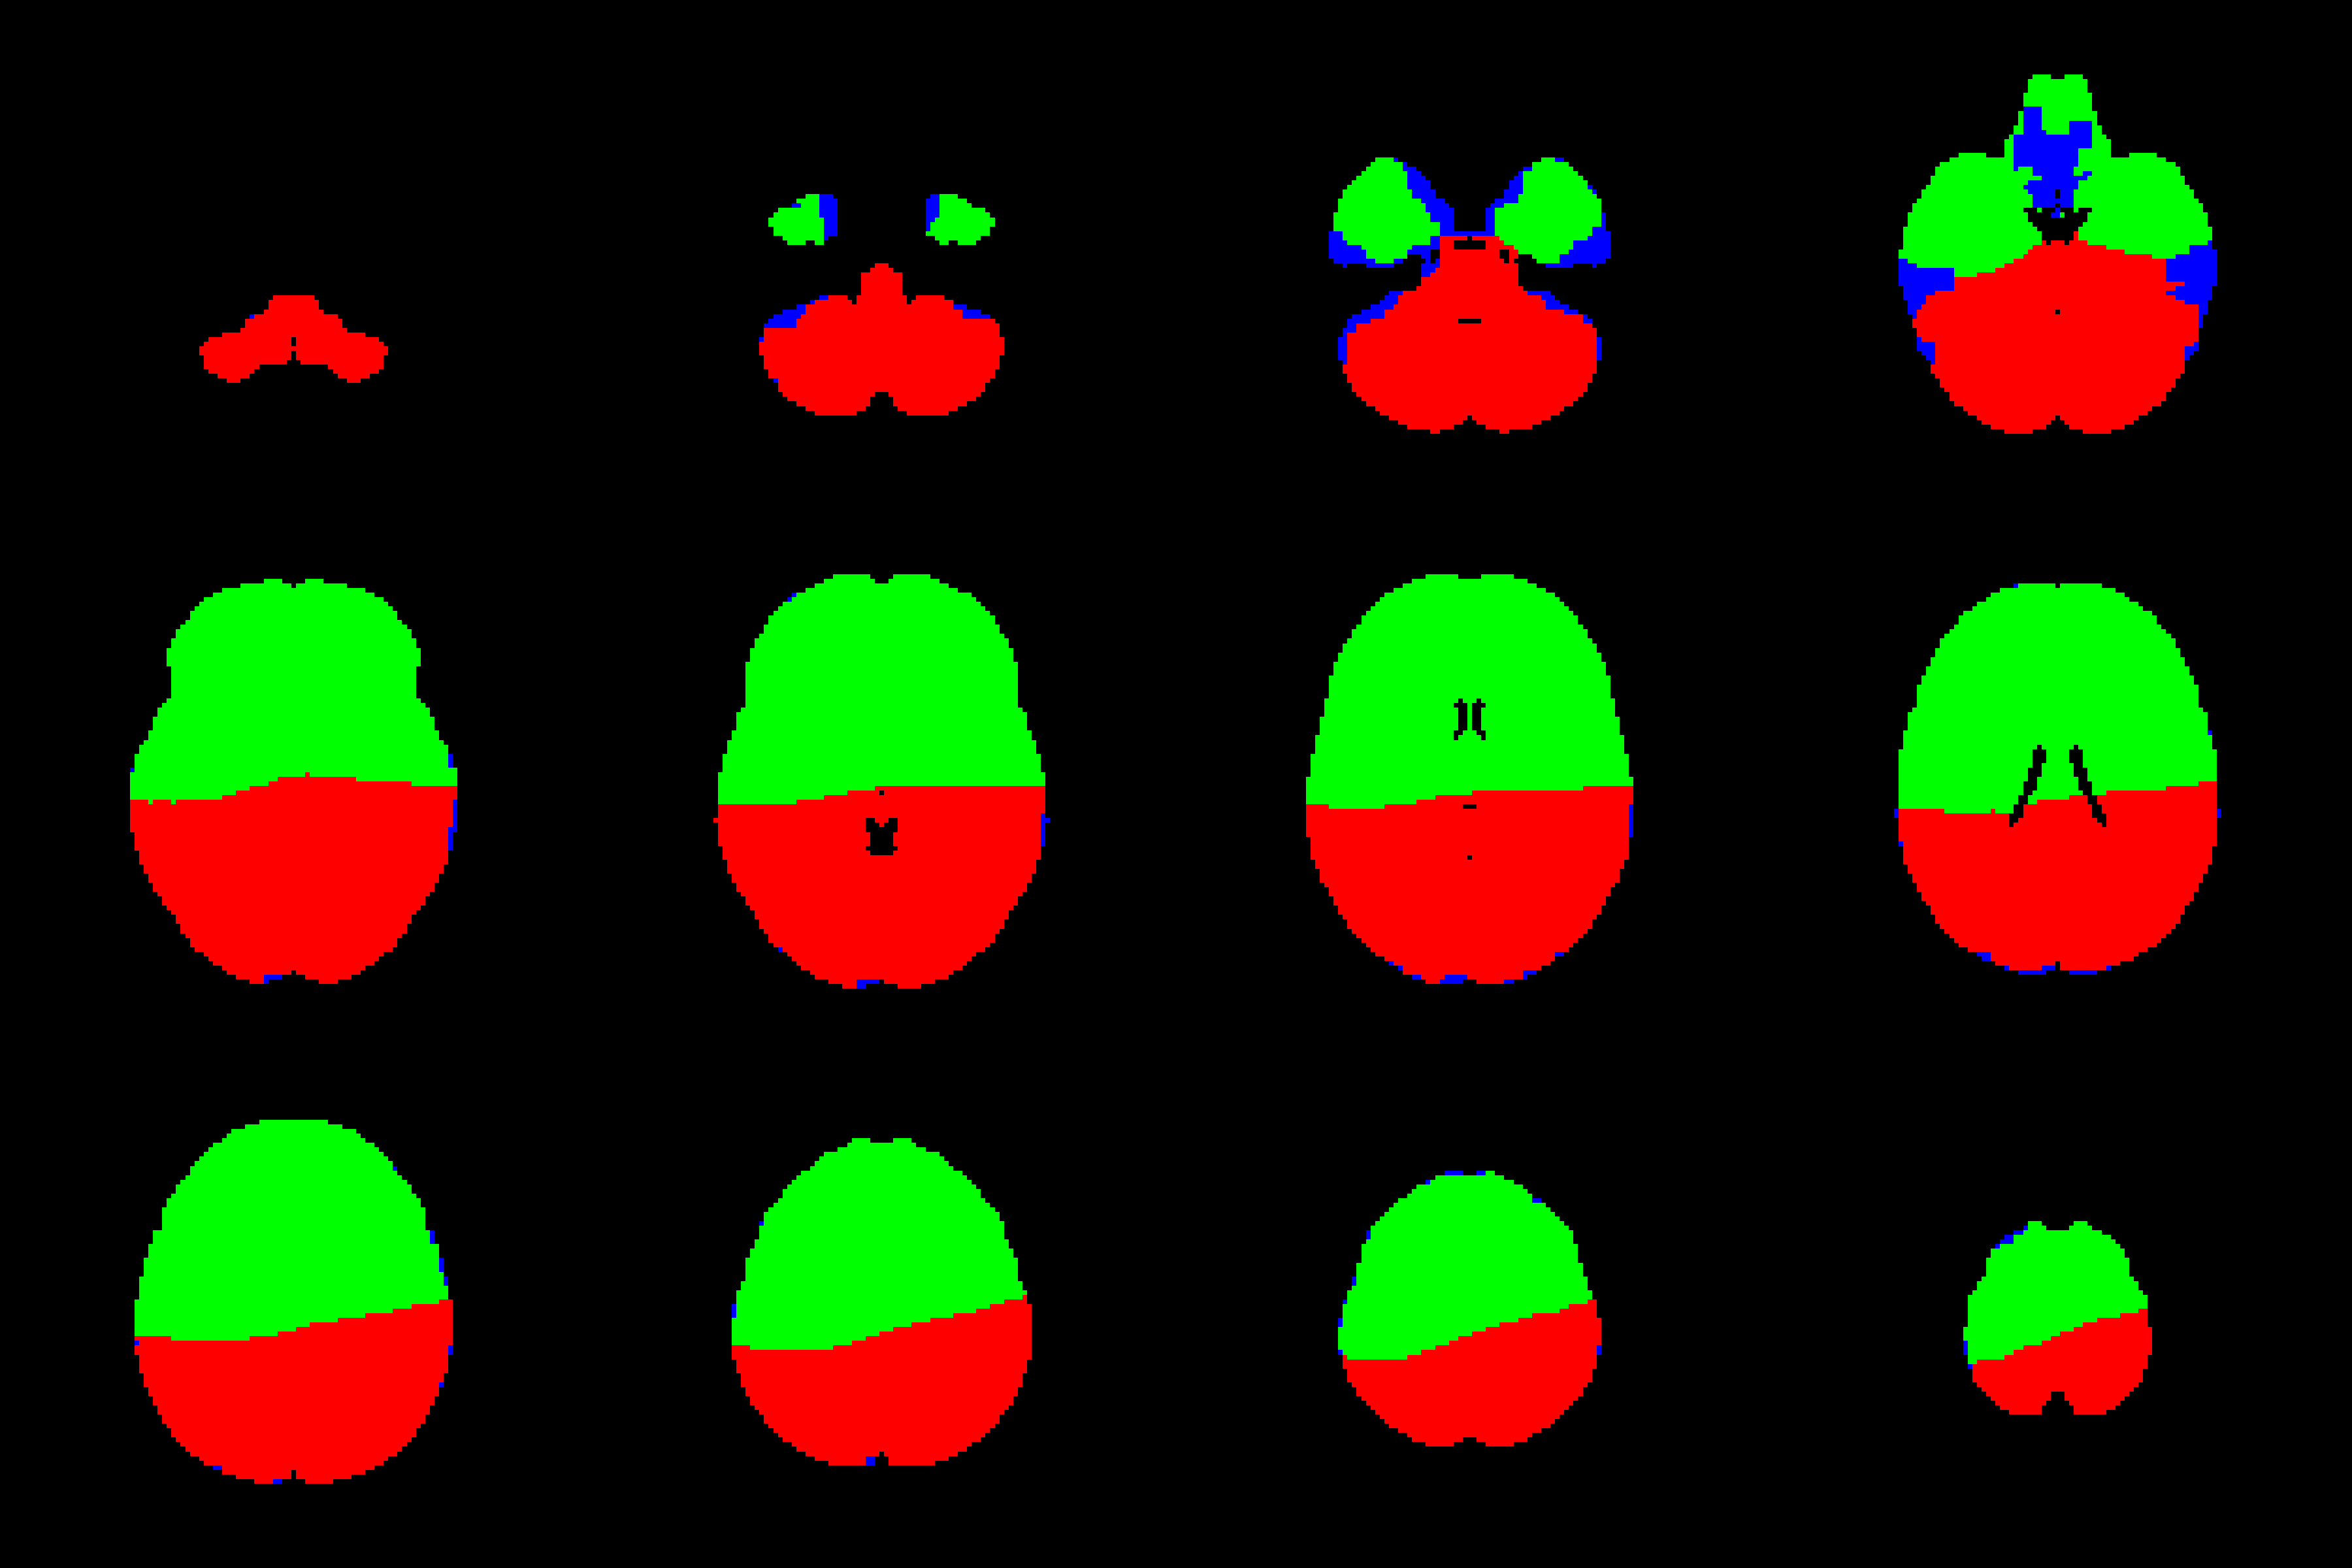
\includegraphics[scale = 0.8]{5_spectral_2_axial.png}

Axial

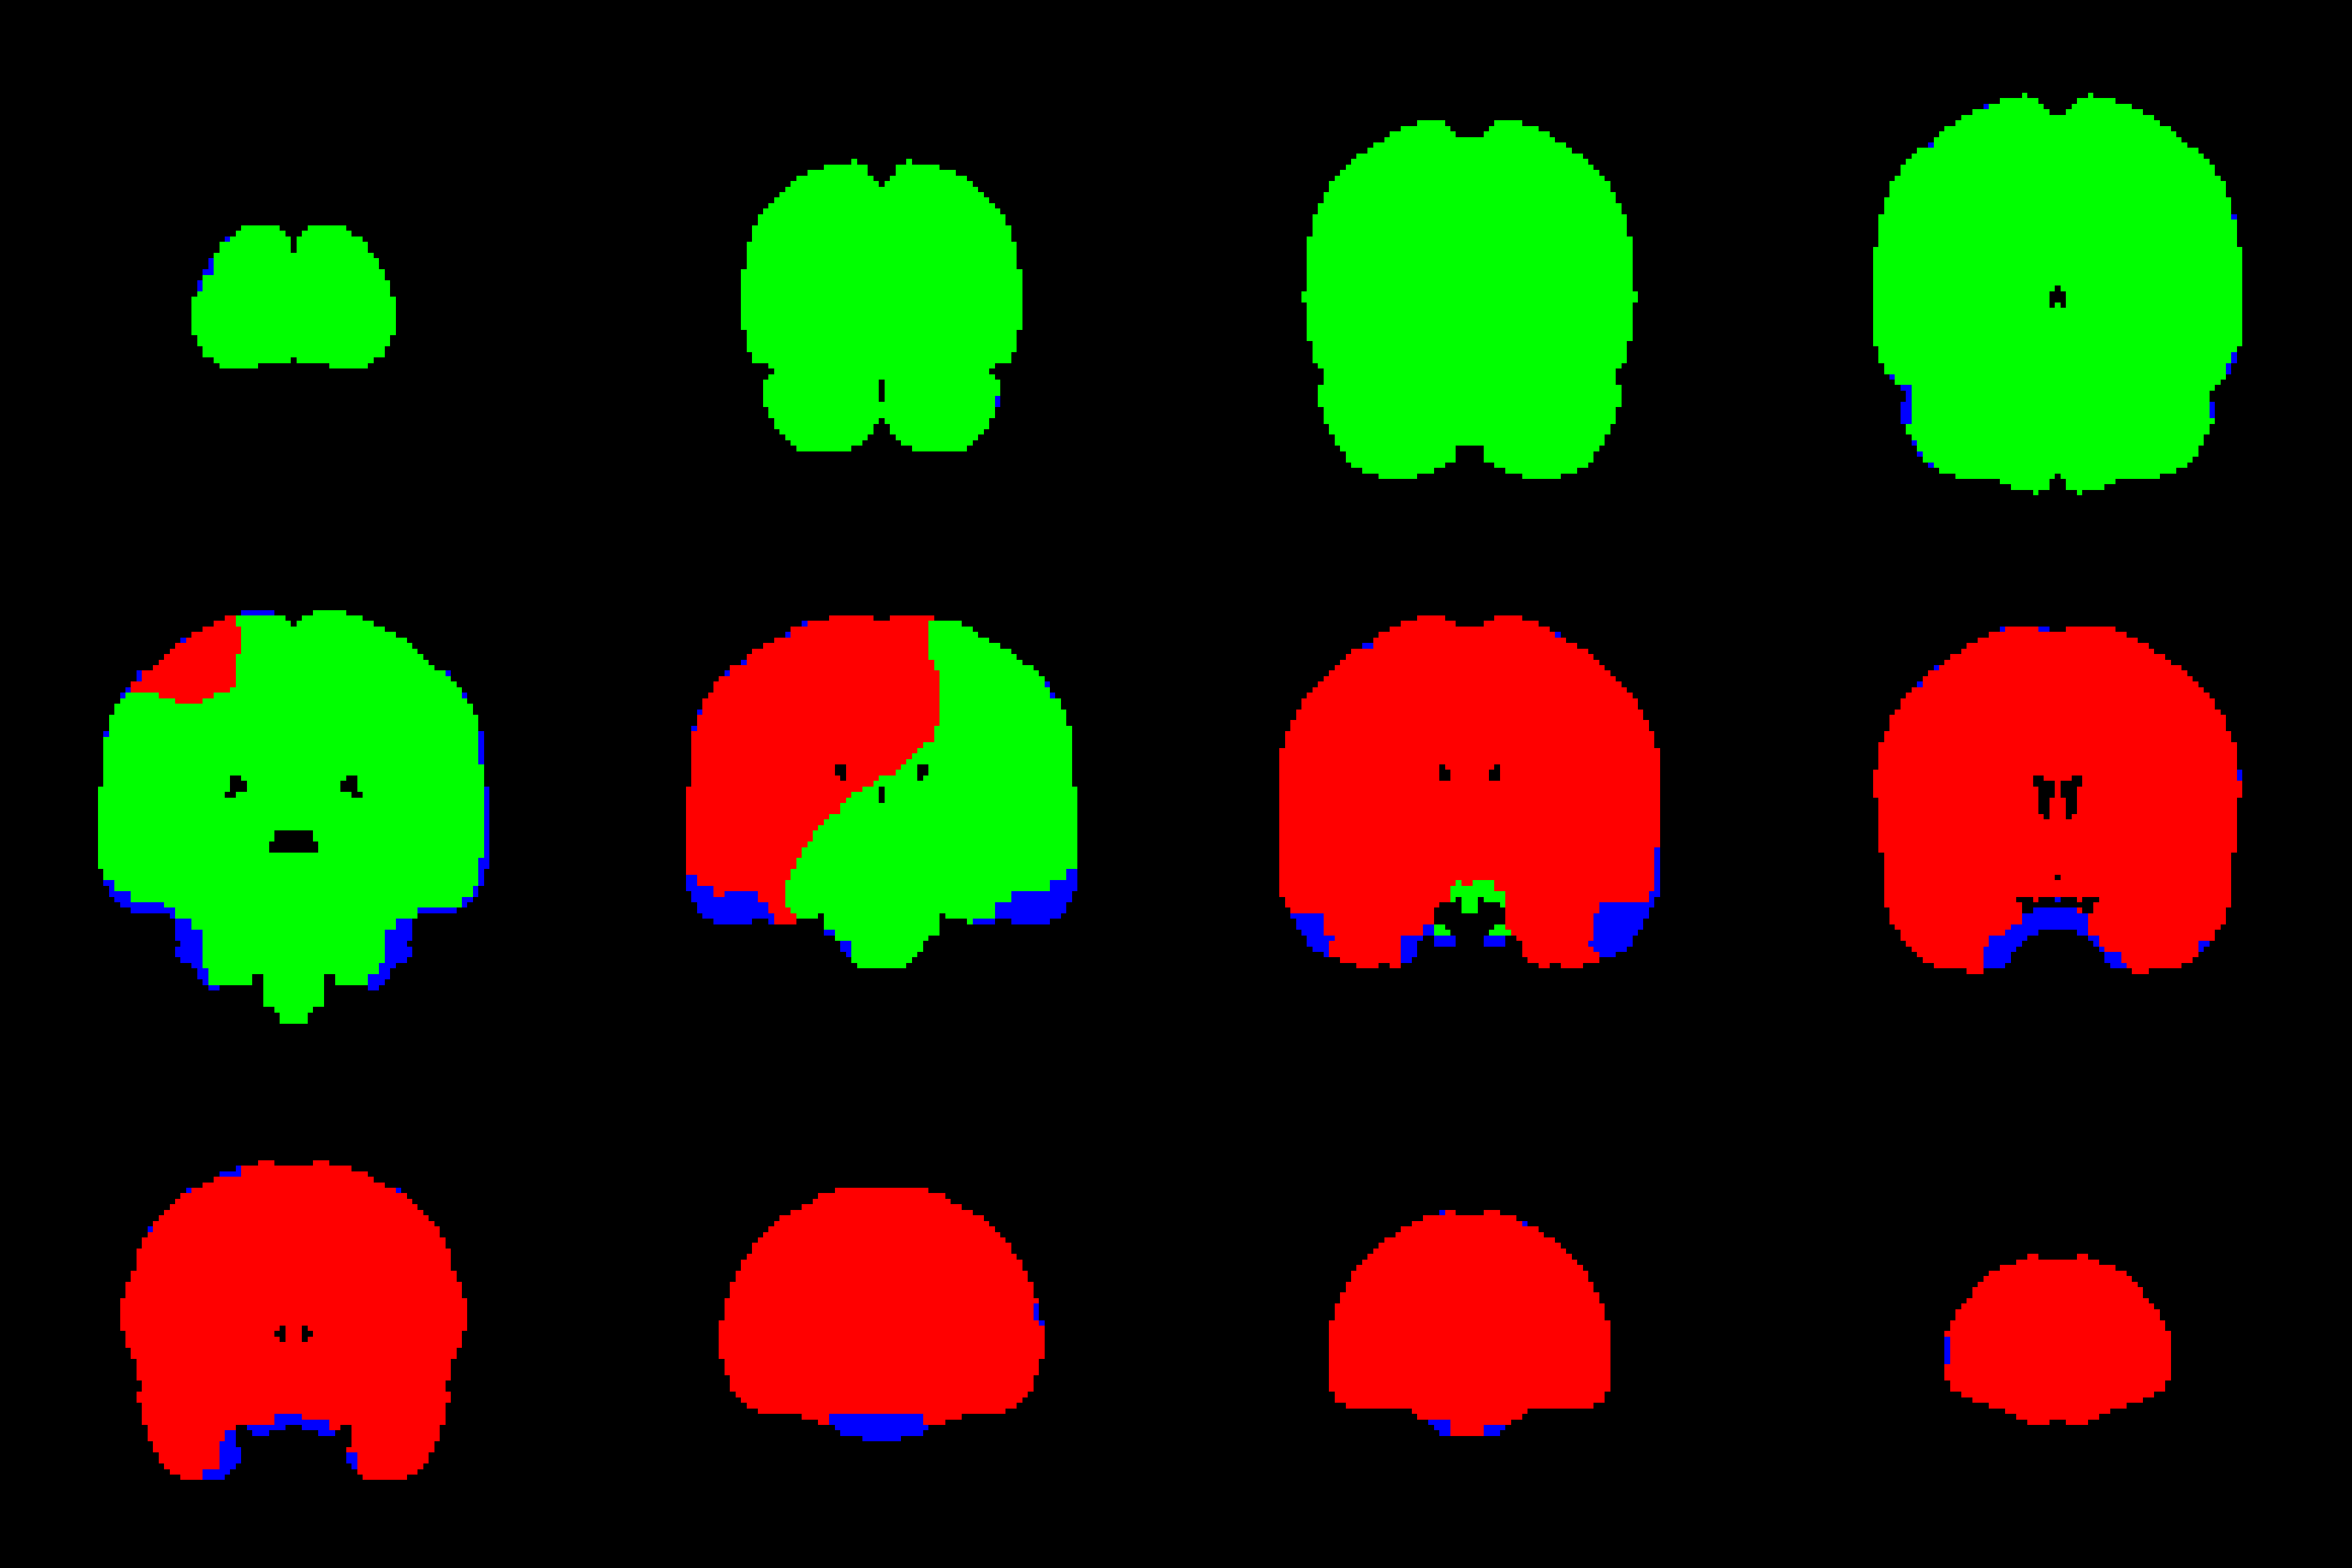
\includegraphics[scale = 0.8]{5_spectral_2_coronal.png}

Coronal

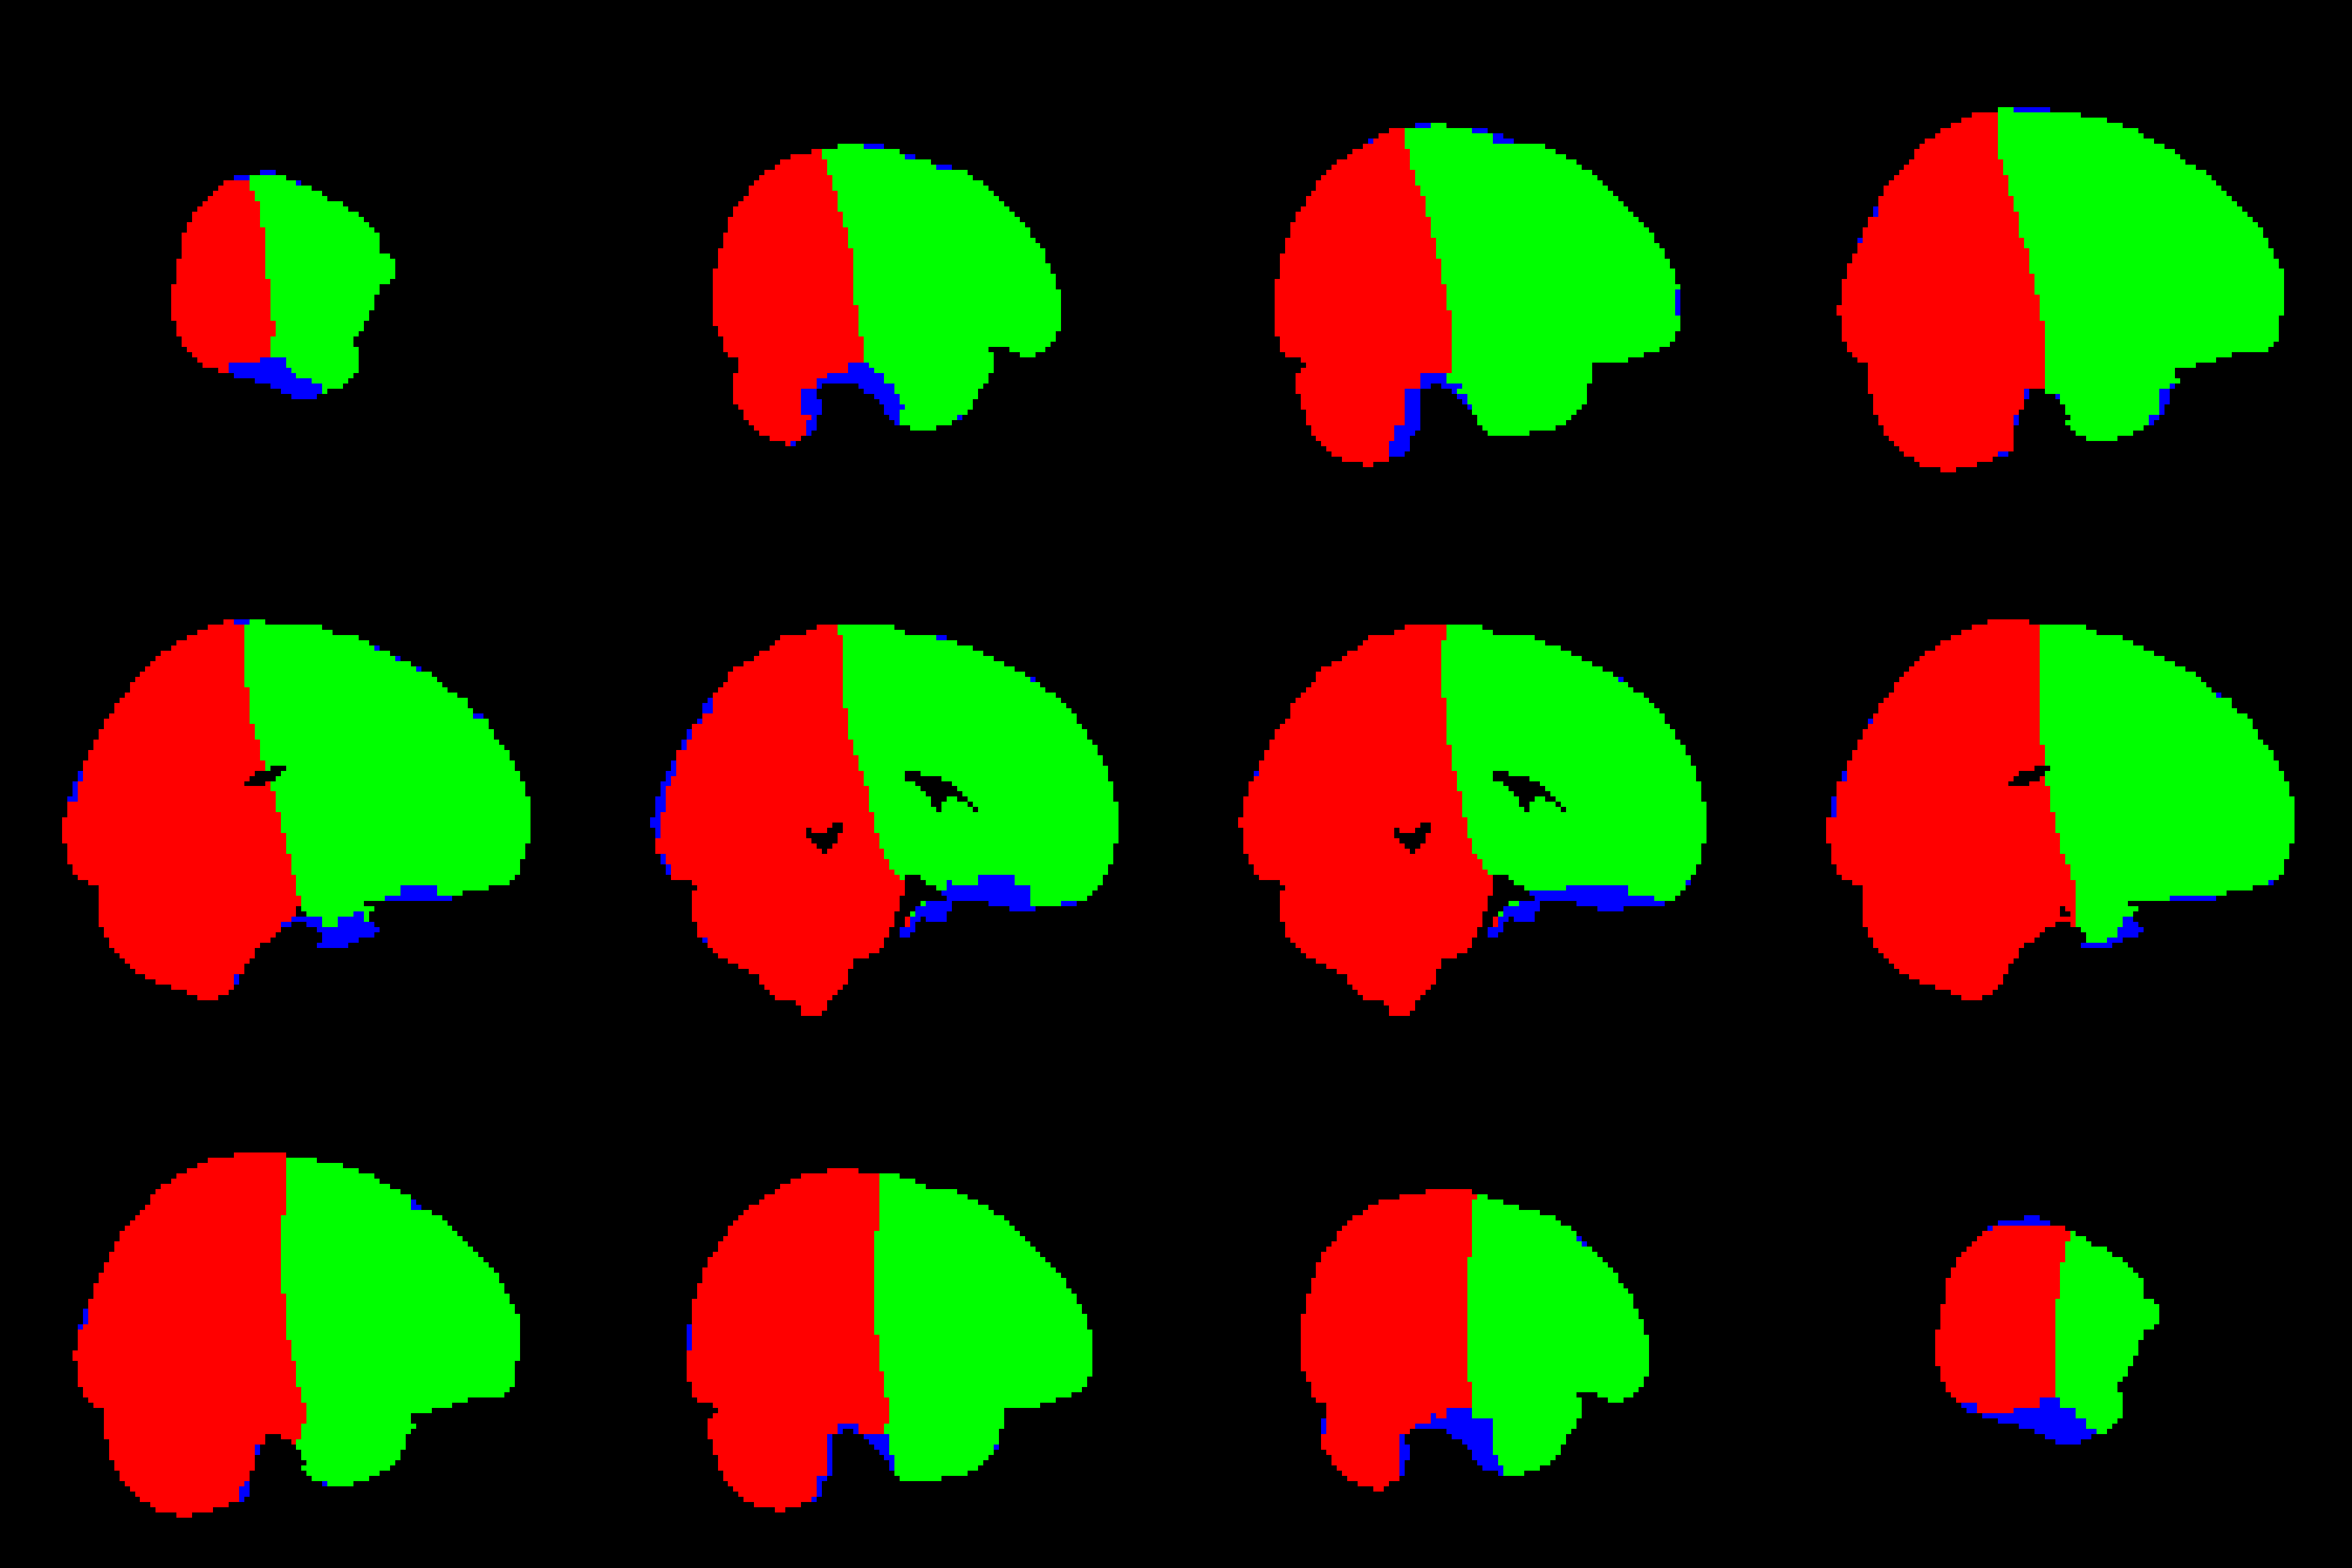
\includegraphics[scale = 0.8]{5_spectral_2_sagittal.png}

Sagittal
\end{center}

As anticipated, the minimum cut approach effectively smoothens the
boundaries of the parcels.

\section{Constrained k-Part Graph Partitioning}

%#######################################################################
